% Chapter 4

\chapter{Experimental Results} % Main chapter title
\label{Chapter4} % For referencing the chapter elsewhere, use \ref{Chapter4} 


%----------------------------------------------------------------------------------------

This chapter describes the results of the experiments. 
%I have made the experience that the accuracy reached depends greatly on the environment. 
On the github repository (\url{https://github.com/JoelNiklaus/IndoLoc/tree/master/app/src/main/assets/thesis/bern/room}) all the datasets  we collected for the experiments are provided for the interested reader.


\section{Attribute Selection}
\label{sec:AttributeSelection}

The information gain denotes the value a certain attribute has for the overall prediction. If an attribute with a high information gain is removed, we can strongly assume that the prediction accuracy will decrease more than when an attribute with a low information gain is removed. Finding out the information gain of each attribute lets us rank the attributes based on their usefulness.

In order to evaluate the information gain (see \cite{Frank2010}) of each attribute on the dataset Bern Rooms (see Section \ref{sec:BernDataset} and on \url{https://github.com/JoelNiklaus/IndoLoc/tree/master/app/src/main/assets/thesis/bern/room}), we run the  InfoGainAttributeEval (see  \url{http://weka.sourceforge.net/doc.dev/weka/attributeSelection/InfoGainAttributeEval.html}) ranking algorithm in Weka, getting the  following result in Table \ref{tab:InfoGain}.

% TABLE
\begin{table}[H]
	\begin{threeparttable}
		\caption{The information gain of each attribute using the InfoGainAttributeEval ranking algorithm.}
		\label{tab:InfoGain}
		\centering
		\begin{tabular}{l r r}
		\toprule
		\tabhead{Attribute Name} & \tabhead{Information Gain} & \tabhead{Attribute Index} \\
		\midrule
light & 2.3540   &  3 \\
latitude & 2.3427  & 16 \\
longitude & 2.1380   & 17 \\
rssValue5 & 1.9490   & 23 \\
rssValue4 & 1.9462  & 22 \\
rssValue3 & 1.9288  & 21 \\
rssValue1 & 1.8435  & 19 \\
rssValue2 & 1.8426  & 20 \\
rssValue6 & 1.8079  & 24 \\
rssValue0 & 1.5762  & 18 \\
rssValue8 & 1.5582  & 26 \\
rssValue9 & 1.4883  & 27 \\
rssValue7 & 1.2531  & 25 \\
geomagneticMagnitude & 0.6001  & 13 \\
magneticProcessedZ & 0.3557  & 15 \\
magneticProcessedY & 0.3459  & 14 \\
gravityMagnitude & 0.0573  & 12 \\
pressure & 0       &  4 \\
magneticZ & 0       & 11 \\
magneticY & 0       & 10 \\
relativeHumidity & 0       &  5 \\
gravityX & 0       &  6 \\
gravityY & 0       &  7 \\
gravityZ & 0       &  8 \\
magneticX & 0       &  9 \\
ambientTemperature & 0       &  2 \\
			\bottomrule\\
		\end{tabular}
		\begin{tablenotes}
      \small
      \item Dataset Bern Rooms (see Section \ref{sec:BernDataset} and on \url{https://github.com/JoelNiklaus/IndoLoc/tree/master/app/src/main/assets/thesis/bern/room}).
    \end{tablenotes}
	\end{threeparttable}
\end{table}


This ranking provides information about the probable importance of the features. The top ranked feature contains the greatest information gain and is therefore probably very important for the predictions made by the classifiers used later on.
The 9 features at the bottom of the ranking have an information gain of 0. Therefore, we already know that these 9 attributes are only cluttering the data and are of no use to us. So we can already delete these out of the dataset. This results in no difference in accuracy but in a decrease in both training and testing time as the algorithms have to consider less data.


%----------------------------------------------------------------------------------------








%\section{One Dataset}
%
%The \href{https://github.com/JoelNiklaus/IndoLoc/blob/master/app/src/test/java/ch/joelniklaus/indoloc/experiments/OneDatasetTest.java}{One Dataset Test} checks if the accuracy is increased when the data points are reshuffled. So the training and testing dataset are merged together and then randomly redistributed to the training and testing dataset. This should be no problem and should not change the result at all. But here the following big mystery occurs:
%
%% TABLE
%\begin{table}
%	\begin{threeparttable}
%		\caption{The accuracy change if the data points are redistributed.}
%		\label{tab:OneDataset}
%		\centering
%		\begin{tabular}{l r r}
%		\toprule
%		\tabhead{Classifier} & \tabhead{Original Datasets} & \tabhead{Merged and redistributed} \\
%		\midrule
%		MultilayerPerceptron	& 91.41 & 88.90 \\%		SMO						& 89.90 & 92.88 \\%		Logistic				& 89.29 & 92.88 \\%		NaiveBayes				& 82.12 & 91.19 \\%		IBk						& 79.49 & 98.67 \\%		RandomForest			& 79.49 & 99.16 \\%		J48						& 75.45 & 97.59 \\
%		\bottomrule\\
%		\end{tabular}
%		\begin{tablenotes}
%      \small
%      \item Dataset: \href{https://github.com/JoelNiklaus/IndoLoc/tree/master/app/src/main/assets/thesis/exeter/landmark}{Exeter Landmarks}
%    \end{tablenotes}
%	\end{threeparttable}
%\end{table} \\
%
%% CHART
%\begin{figure}[th]
%\centering
%\includegraphics[width=150mm]{Figures/oneDataset.png}
%\decoRule
%\caption[OneDataset]{Original and redistributed data points.}
%\label{fig:OneDataset}
%\end{figure}
%
%As we can clearly see in Table \ref{tab:OneDataset} and in a visualized way in Chart \ref{fig:OneDataset}, redistributing the data points somehow makes the prediction almost perfect for some algorithms. RandomForest for instance almost achieves 100\% accuracy. This is very confusing and does not make much sense. In the beginning of the experimental phase I collected only one dataset. I then randomly split this dataset into a training set and a testing set. This is how it is how normally a ML model is evaluated. ADD REFERENCE HERE. Then I got results like this here which were surprisingly good. However when I loaded the model onto the smart phone and tested it live, the accuracy was very bad. So because of this I changed to collecting the training and the testing set separately. Using this approach the live testing accuracy improved. Live testing is very difficult to analyze, therefore I analyze it like this now. The interested reader though is invited to try the live testing using the app available on my \href{https://github.com/JoelNiklaus/IndoLoc}{github repository}.

%----------------------------------------------------------------------------------------


\section{Duplicates Removal}
\label{sec:DuplicatesRemoval}

As described in Section \ref{sec:DataCollection} and depicted in Figure \ref{fig:Grid} there are some intersections in the path covered by the researcher to collect data. At these intersections or at locations very close to each other it is possible that every attribute of two rows in the dataset have the same values. These are denoted as duplicate data points.

The Duplicates Test (on \url{https://github.com/JoelNiklaus/IndoLoc/blob/master/app/src/test/java/ch/joelniklaus/indoloc/experiments/DuplicatesTest.java}) checks if the accuracy is increased when all the duplicate data points are removed. After removing the duplicate data, it is clear that every data point is unique. A data point is a duplicate of another data point if all the correspondent feature values are exactly the same and they belong to the same class - simply put, if both data points are exactly the same.

% TABLE
\begin{table}[H]
	\begin{threeparttable}
		\caption{The accuracy change if duplicate data points are removed.}
		\label{tab:Duplicates}
		\centering
		\begin{tabular}{l r r}
		\toprule
		\tabhead{Classifier} & \tabhead{With Duplicates} & \tabhead{Without Duplicates} \\
		\midrule
								& train set: 2522, testset: 1269 & train set: 1772, testset: 990\\
		MultilayerPerceptron	& 88.42\%	& 91.41\% \\		Logistic				& 85.03\%	& 89.29\% \\		SMO						& 84.87\%	& 89.90\% \\		KStar					& 80.61\%	& 82.83\% \\		J48						& 80.54\%	& 75.45\% \\		RandomForest			& 80.46\%	& 79.49\% \\		NaiveBayes				& 78.33\%	& 82.12\% \\		IBk						& 75.10\%	& 79.49\% \\
		\bottomrule\\
		\end{tabular}
		\begin{tablenotes}
      \small
      \item Dataset Exeter Landmarks (see Section \ref{sec:ExeterDataset} and on \url{https://github.com/JoelNiklaus/IndoLoc/tree/master/app/src/main/assets/thesis/exeter/landmark}).
    \end{tablenotes}
	\end{threeparttable}
\end{table} 

% CHART
\begin{figure}[H]
\centering
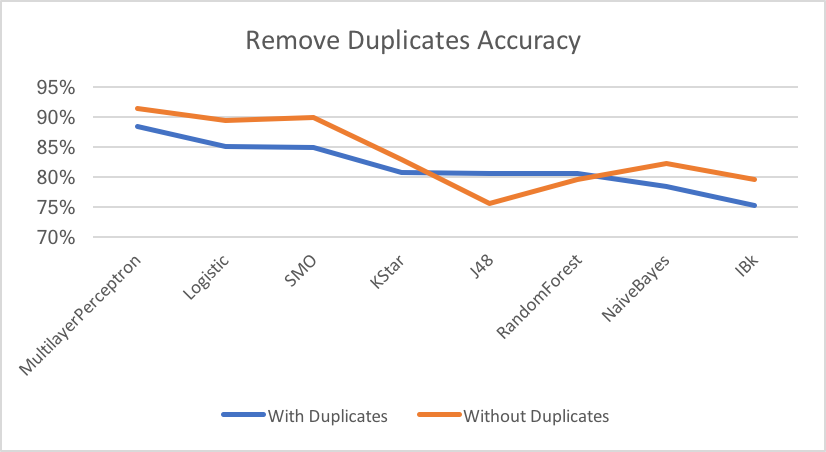
\includegraphics[width=150mm]{Figures/Duplicates.png}
\decoRule
\caption[Duplicates]{Landmark prediction accuracy with and without duplicate data points. Dataset Exeter Landmarks (see Section \ref{sec:ExeterDataset} and on \url{https://github.com/JoelNiklaus/IndoLoc/tree/master/app/src/main/assets/thesis/exeter/landmark})}
\label{fig:Duplicates}
\end{figure}

As we can clearly see in Table \ref{tab:Duplicates} and in a visualized way in Figure \ref{fig:Duplicates}, removing duplicate values increases the accuracy for most of the algorithms and especially for the ones that perform well. Of course, the computation time is decreased because the ML methods have less data points to consider. As a consequence, for all the following experiments duplicate values are removed.

We can see that after removing the duplicates the Multilayer Perceptron reaches a maximum landmark prediction accuracy of 91.41\%.

%----------------------------------------------------------------------------------------


%\section{Smaller Dataset}
%The \href{https://github.com/JoelNiklaus/IndoLoc/blob/master/app/src/test/java/ch/joelniklaus/indoloc/experiments/SmallerDataSetTest.java}{Smaller Dataset Test} checks if the accuracy is increased when only a randomly selected smaller part of the dataset is used. If this is the case, of course the performance is increased as well, because less data points have to be evaluated by the ML methods.
%
%
%
%% TABLE
%\begin{table}
%	\begin{threeparttable}
%		\caption{The accuracy change with randomly selected smaller datasets.}
%		\label{tab:SmallerDataset}
%		\centering
%		\begin{tabular}{l r r r r r r r}
%		\toprule
%		\tabhead{Classifier} & \tabhead{Full} & \tabhead{Half} & \tabhead{Third} & \tabhead{Fourth} & \tabhead{Fifth}  & \tabhead{Tenth} & \tabhead{Twentieth} \\
%		\midrule
%		MultilayerPerceptron		&	91.41\%	&	91.92\%	&	90.91\%	&	89.52\%	&	90.40\%	&	78.79\%	&	68.00\% \\%SMO	&	89.90\%	&	89.09\%	&	90.61\%	&	87.90\%	&	90.40\%	&	88.89\%	&	94.00\% \\%Logistic	&	89.29\%	&	88.89\%	&	90.61\%	&	88.71\%	&	88.89\%	&	80.81\%	&	90.00\% \\%NaiveBayes	&	82.12\%	&	80.61\%	&	83.03\%	&	82.26\%	&	85.35\%	&	90.91\%	&	92.00\% \\%IBk	&	79.49\%	&	77.78\%	&	80.61\%	&	78.23\%	&	79.80\%	&	77.78\%	&	88.00\% \\%RandomForest	&	79.49\%	&	79.80\%	&	83.03\%	&	82.66\%	&	83.33\%	&	81.82\%	&	90.00\% \\%J48	&	75.45\%	&	74.95\%	&	74.55\%	&	81.85\%	&	77.78\%	&	85.86\%	&	74.00\% \\
%		\bottomrule\\
%		\end{tabular}
%		\begin{tablenotes}
%      \small
%      \item Dataset: \href{https://github.com/JoelNiklaus/IndoLoc/tree/master/app/src/main/assets/thesis/exeter/landmark}{Exeter Landmarks}
%    \end{tablenotes}
%	\end{threeparttable}
%\end{table} \\
%
%% CHART
%\begin{figure}[th]
%\centering
%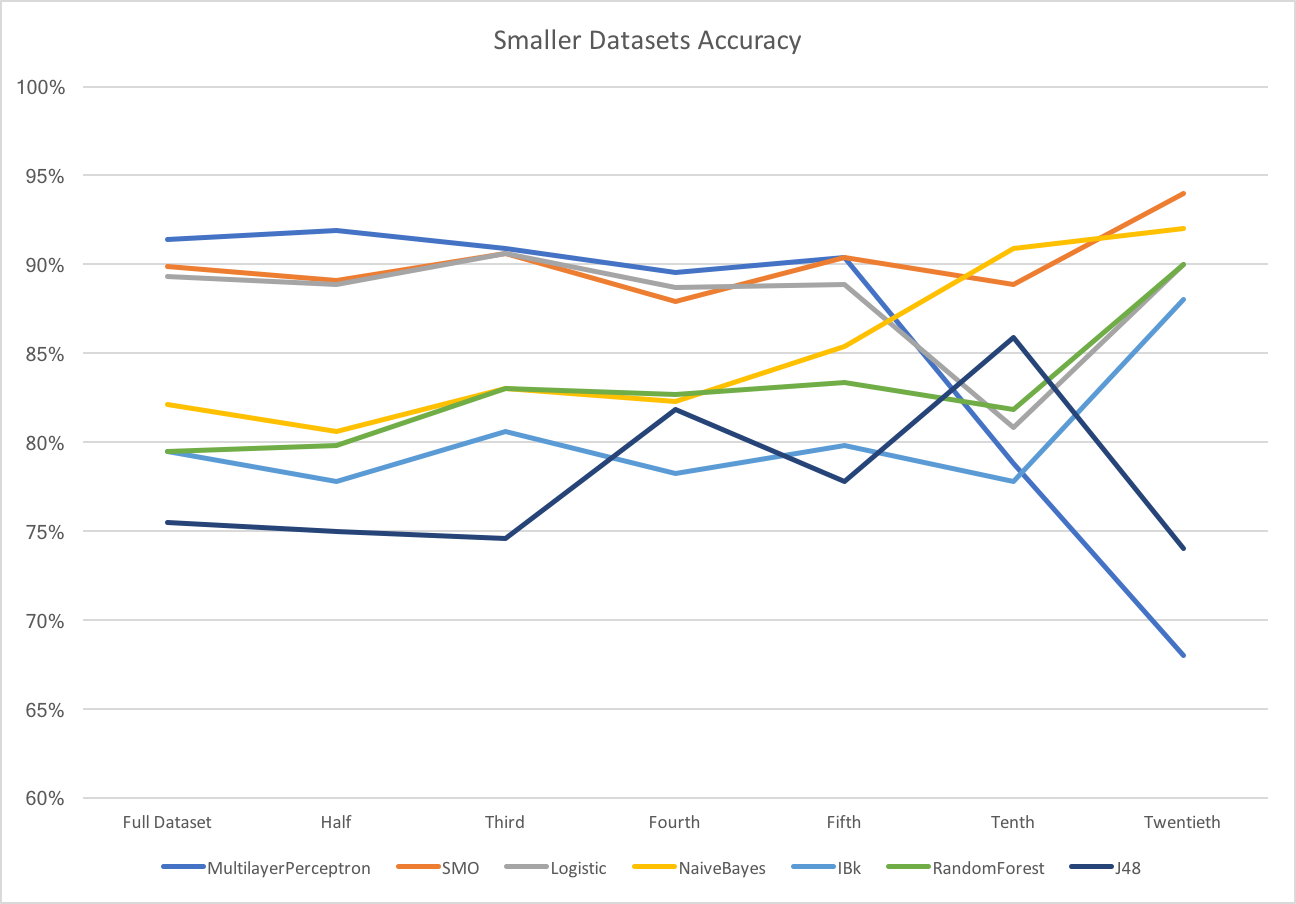
\includegraphics[width=150mm]{Figures/SmallerDataset.png}
%\decoRule
%\caption[SmallerDataset]{The accuracy change with randomly selected smaller datasets.}
%\label{fig:SmallerDataset}
%\end{figure}
%
%As we can see in Table \ref{tab:SmallerDataset} and Chart \ref{fig:SmallerDataset} the prediction accuracy is more or less stable until one third of the original size. In one fourth and one fifth of the size the accuracy decreases slightly. In one tenth and one twentieth of the size it starts to get erratic. So it probably depends on which data points are picked out of the original dataset. So for this dataset I would recommend to use one third of the data to slightly decrease the training and testing time. But the effect is minimal. 


%----------------------------------------------------------------------------------------

\section{Attribute Exclusion}
\label{sec:AttributeExclusion}

In Section \ref{sec:Features} we discussed which features seem reasonable to include into the dataset and which should be omitted because they do not seem helpful. In this section we test if the chosen features really all contribute to the prediction accuracy. To observe this, we selectively excluded certain features and studied the influences on the prediction accuracy.

This is done in the Attribute Exclusion Test (on  \url{https://github.com/JoelNiklaus/IndoLoc/blob/master/app/src/test/java/ch/joelniklaus/indoloc/experiments/AttributeExclusionTest.java}).

\subsection{Only RSS Values}

\subsubsection{Accuracy}


% TABLE
\begin{table}[H]
	\begin{threeparttable}
		\caption{The accuracy with a different number of RSS values.}
		\label{tab:RSSAccuracy}
		\centering
		\begin{tabular}{l r r r r r r}
		\toprule
		\tabhead{Classifier} & \tabhead{5 RSS} & \tabhead{6 RSS} & \tabhead{7 RSS} & \tabhead{8 RSS} & \tabhead{9 RSS}  & \tabhead{10 RSS} \\
		\midrule
		
		
		NaiveBayes &	82.05\%	&79.49\%	&	82.05\%	&	80.77\%	&	84.62\%	&	79.49\% \\IBk &	76.92\%	&	76.92\%	&	82.05\%	&	79.49\%	&	82.05\%	&	75.64\% \\KStar &	75.64\%	&	75.64\%	&	83.33\%	&	78.21\%	&	79.49\%	&	74.36\% \\SMO &	74.36\%	&	70.51\%	&	82.05\%	&	79.49\%	&	78.21\%	&	76.92\% \\Logistic &	73.08\%	&	66.67\%	&	73.08\%	&	66.67\%	&	71.79\%	&	69.23\% \\RandomForest &	71.79\%	&	71.79\%	&	79.49\%	&	75.64\%	&	73.08\%	&	75.64\% \\J48 &	64.10\%	&	57.69\%	&	64.10\%	&	64.10\%	&	64.10\%	&	64.10\% \\MultilayerPerceptron &	42.31\%	&	42.31\%	&	43.59\%	&	48.72\%	&	46.15\%	&	44.87\% \\
		\bottomrule\\
		\end{tabular}
		\begin{tablenotes}
      \small
      \item Dataset Bern Rooms (see Section \ref{sec:BernDataset} and on \url{https://github.com/JoelNiklaus/IndoLoc/tree/master/app/src/main/assets/thesis/bern/room}).
    \end{tablenotes}
	\end{threeparttable}
\end{table} 

% CHART
\begin{figure}[H]
\centering
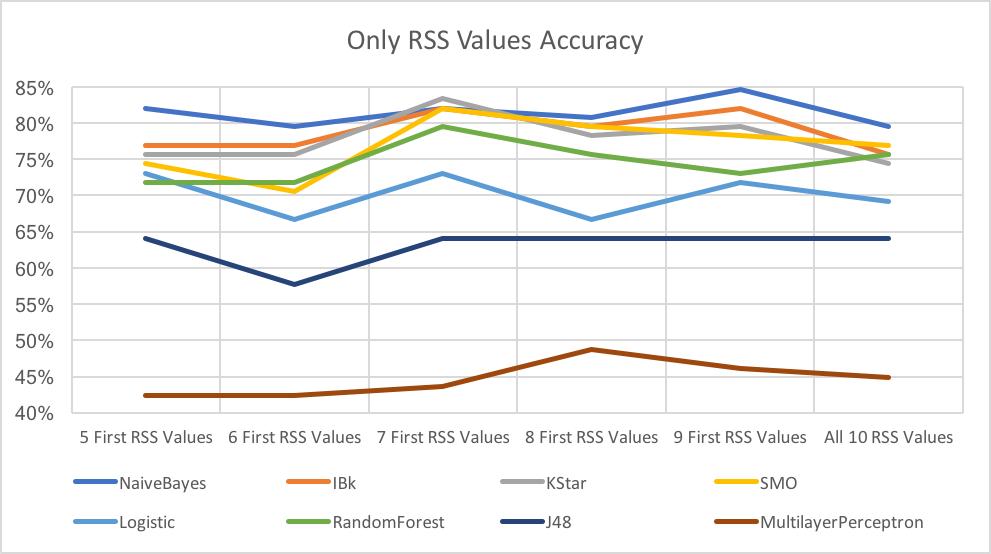
\includegraphics[width=150mm]{Figures/RssAccuracy.png}
\decoRule
\caption[RSSAccuracy]{The accuracy with a different number of RSS values. Dataset Bern Rooms (see Section \ref{sec:BernDataset} and on \url{https://github.com/JoelNiklaus/IndoLoc/tree/master/app/src/main/assets/thesis/bern/room})}
\label{fig:RSSAccuracy}
\end{figure}



Table \ref{tab:RSSAccuracy} and Figure \ref{fig:RSSAccuracy} show that there are two peaks, namely when 7 and 9 RSS values are used. The Naive Bayes classifier reaches a maximum prediction accuracy of 84.62\% with 9 RSS values. The other methods that perform well (KStar, SMO, Logistic and Randomforest) are considerably better with 7 RSS values. Table \ref{tab:RSSTestTime} depicts that there is not a great difference in testing time between 7 and 9 RSS values. Both would be viable options, but because more methods performed well with 7 RSS values and because Naive Bayes was never the best classifier on the final set in our tests, we are working with 7 RSS values in this dataset from now on.
We opine that signal interference may be the reason for worse performance when more than 7 RSS values are utilized.



\subsubsection{Testing Time}


% TABLE
\begin{table}[H]
	\begin{threeparttable}
		\caption{The testing time with a different number of RSS values measured in \textmu s per instance.}
		\label{tab:RSSTestTime}
		\centering
		\begin{tabular}{l r r r r r r}
		\toprule
		\tabhead{Classifier} & \tabhead{5 RSS} & \tabhead{6 RSS} & \tabhead{7 RSS} & \tabhead{8 RSS} & \tabhead{9 RSS}  & \tabhead{10 RSS} \\
		\midrule
		
		
		
NaiveBayes	&	108	&	201	&	150	&	106	&	83	&	173 \\IBk	&	283	&	231	&	262	&	230	&	294	&	297 \\KStar	&	863	&	1747	&	1095	&	1139	&	1285	&	1633 \\SMO	&	58	&	55	&	63	&	45	&	62	&	63 \\Logistic	&	20	&	24	&	21	&	22	&	23	&	28 \\RandomForest	&	31	&	39	&	46	&	20	&	38	&	34 \\J48	&	20	&	25	&	59	&	25	&	22	&	23 \\MultilayerPerceptron	&	9	&	10	&	11	&	10	&	7	&	12 \\
		
		\bottomrule\\
		\end{tabular}
		\begin{tablenotes}
      \small
      \item Dataset Bern Rooms (see Section \ref{sec:BernDataset} and on \url{https://github.com/JoelNiklaus/IndoLoc/tree/master/app/src/main/assets/thesis/bern/room}).
    \end{tablenotes}
	\end{threeparttable}
\end{table} 


% CHART
\begin{figure}[H]
\centering
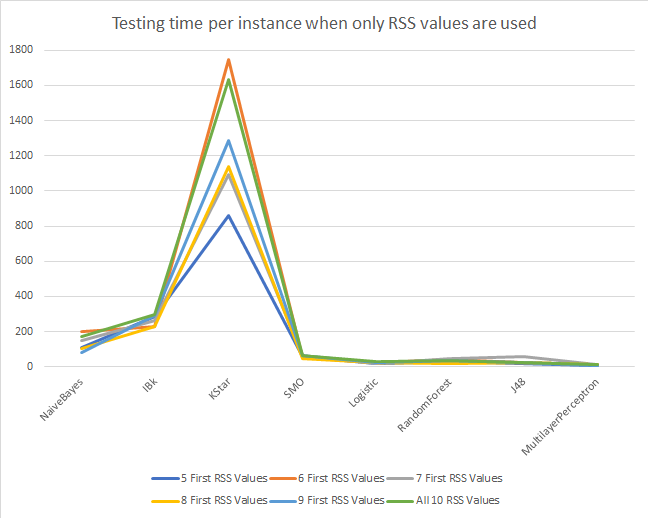
\includegraphics[width=150mm]{Figures/RssTestTime.png}
\decoRule
\caption[RSS Testing Time]{The testing time with a different number of RSS values measured in \textmu s per instance. Dataset Bern Rooms (see Section \ref{sec:BernDataset} and on \url{https://github.com/JoelNiklaus/IndoLoc/tree/master/app/src/main/assets/thesis/bern/room}).}
\label{fig:RSSTestTime}
\end{figure}

Testing time is defined as the time needed to classify an instance and is measured in \textmu s per instance. The tests have been conducted on a MacBook Pro, late 2013 edition with a 2.4 GHz Intel Core i5 CPU running macOS Sierra .

Table \ref{tab:RSSTestTime} and Figure \ref{fig:RSSTestTime} present that instance based methods like IBk (K-Nearest Neighbour) and especially KStar need so much more time than the other methods (IBk between 230 and 297 and KStar between 863 and 1747 microseconds per instance). This is because they have to look at the whole dataset each time an instance is classified, in contrast to other methods that use functions whose parameters are tweaked during the training phase. As a consequence, we excluded KStar from these big datasets (room recognition), because the experiment would take too long, which is not practical in a real scenario. However, for landmark recognition it makes sense to include it, because the datasets are normally much smaller.
The best testing time was achieved by the Multilayer Perceptron with predictions made in between 7 and 12 microseconds per instance.



%ANDERES PAPER ZITIEREN 





\subsection{RSS and Magnetic Field}

This section describes how the room prediction accuracy changes when we add the magnetic field (see Section \ref{sec:MagneticField}), stored in different ways, to the RSS values. 

% TABLE
\begin{table}[H]
	\begin{threeparttable}
		\caption{The accuracy with different ways of storing the magnetic field.}
		\label{tab:RSSAndMagnetic}
		\centering
		\begin{tabular}{l r r r r r}
		\toprule
		\tabhead{Classifier} & \tabhead{1} & \tabhead{2} & \tabhead{3} & \tabhead{4} & \tabhead{5} \\
		\midrule
		
SMO &	82.05\%	&	82.05\%	&	87.51\%	&	88.06\%	&	86.98\% \\IBk	& 82.05\%	&	82.05\%	&	85.57\%	&	85.21\%	&	83.71\% \\NaiveBayes	&	82.05\%	&	82.05\%	&	82.82\%	&	80.94\%	&	79.99\% \\RandomForest	&	79.49\%	&	78.21\%	&	78.22\%	&	80.89\%	&	72.25\% \\Logistic	&	73.08\%	&	73.08\%	&	78.64\%	&	68.62\%	&	73.21\% \\J48	&	64.1\%	&	64.10\%	&	71.27\%	&	71.27\%	&	71.27\% \\MultilayerPerceptron	&	43.59\%	&	39.74\%	&	68.30\%	&	68.40\%	&	79.81\% \\
		
		\bottomrule\\
		\end{tabular}
	\begin{tablenotes}
      \small
      \item Dataset Bern Rooms (see Section \ref{sec:BernDataset} and on \url{https://github.com/JoelNiklaus/IndoLoc/tree/master/app/src/main/assets/thesis/bern/room}).
        \item Legend:
\item[1] 7 first RSS values
\item[2] RSS and gravityRaw and magneticRaw
\item[3] RSS and magneticProcessed
\item[4] RSS and gravityMagnitude and geomagneticMagnitude
\item[5] RSS and magneticProcessed and gravityMagnitude and geomagneticMagnitude
      
    \end{tablenotes}
	\end{threeparttable}
\end{table} 

% CHART
\begin{figure}[H]
\centering
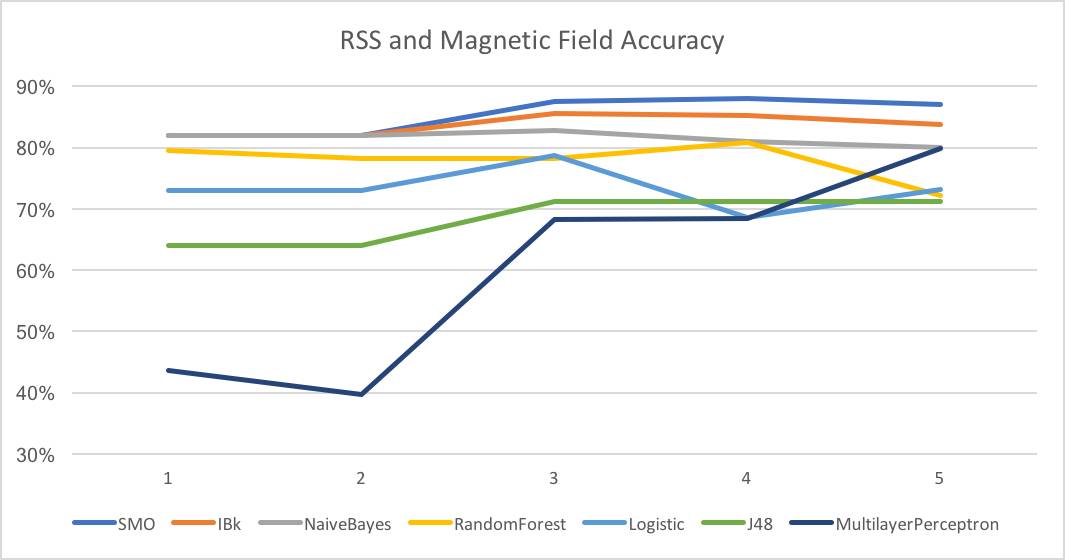
\includegraphics[width=150mm]{Figures/RSSAndMagnetic.png}
\decoRule
\caption[RSSAndMagnetic]{The accuracy with different ways of storing the magnetic field. Dataset Bern Rooms (see Section \ref{sec:BernDataset} and on \url{https://github.com/JoelNiklaus/IndoLoc/tree/master/app/src/main/assets/thesis/bern/room}).}
\label{fig:RSSAndMagnetic}
	
	\begin{threeparttable}
    \begin{tablenotes}
  \item Legend:
\item[1] 7 RSS values
\item[2] RSS and gravityRaw and magneticRaw
\item[3] RSS and magneticProcessed
\item[4] RSS and gravityMagnitude and geomagneticMagnitude
\item[5] RSS and magneticProcessed and gravityMagnitude and geomagneticMagnitude
    \end{tablenotes}
	\end{threeparttable}

\end{figure}


%TABLES AND CHARTS SHOULD APPEAR AT THE RIGHT PLACE

%EXPLAIN HOW EXACTLY VALUES ARE COMPUTED VERWEIS AUF THEORIE

Table \ref{tab:RSSAndMagnetic} and Figure \ref{fig:RSSAndMagnetic} indicate that adding the raw values of the gravity and magnetic field (2) does not improve the accuracy . Adding the magneticProcessed values (3) improves prediction accuracy for most of the algorithms and by 5\% for the best performing method SMO (Sequential Minimal Optimization), for example. Adding the gravity magnitude and the geomagnetic magnitude instead of magneticProcessed (4), some methods perform better and some worse. SMO for instance still improves, but Logistic Regression gets worse. Adding both of the last two at the same time, (5) we could expect that the effect is combined. But interestingly, the accuracy of the top performing methods decreases again. On the other hand, the MultilayerPerceptron performs much better. 
The best room prediction accuracy is reached by the SMO classifier with 88.06\% using RSS values, gravityMagnitude and geomagneticMagnitude




\subsection{Additional Features}
\label{AdditionalFeatures}

This section describes how the room prediction accuracy changes, when we add additional features, namely light and GPS data, to the dataset.

% TABLE
\begin{table}[H]
	\begin{threeparttable}
		\caption{The accuracy with additional features added.}
		\label{tab:AdditionalFeatures}
		\centering
		\begin{tabular}{l r r r}
		\toprule
		\tabhead{Classifier} & \tabhead{1} & \tabhead{2} & \tabhead{3} \\
		\midrule
		
SMO &	86.98\%	&	88.02\%	&	84.16\% \\IBk	& 83.71\%	&	84.74\%	&	81.1\% \\NaiveBayes &	79.99\%	&	90.13\%	&	44.12\% \\MultilayerPerceptron &	79.81\%	&	73.16\%	&	44.93\% \\Logistic &	73.21\%	&	71.81\%	&	55.77\% \\RandomForest &	72.25\%	&	82.33\%	&	41.55\% \\J48 &	71.27\%	&	76.57\%	&	35.65\% \\
				
		\bottomrule\\
		\end{tabular}
		\begin{tablenotes}
      \small
      \item Dataset Bern Rooms (see Section \ref{sec:BernDataset} and on \url{https://github.com/JoelNiklaus/IndoLoc/tree/master/app/src/main/assets/thesis/bern/room}).
      \item Legend:
      \item[1] RSS and magneticProcessed and gravityMagnitude and geomagneticMagnitude
\item[2] RSS and magneticProcessed and gravityMagnitude and geomagneticMagnitude and Light
\item[3] RSS and magneticProcessed and gravityMagnitude and geomagneticMagnitude and Latitude and Longitude
    \end{tablenotes}
	\end{threeparttable}
\end{table} 

% CHART
\begin{figure}[H]
\centering
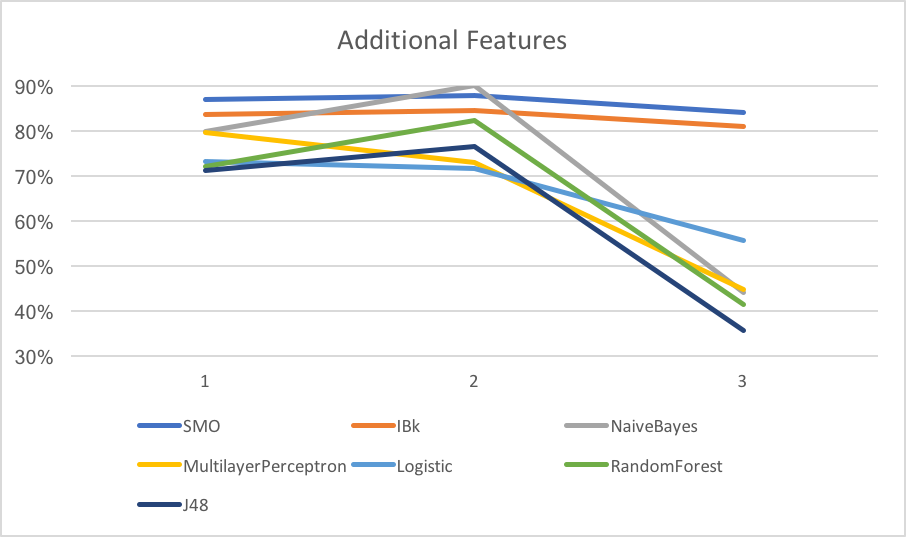
\includegraphics[width=150mm]{Figures/AdditionalFeatures.png}
\decoRule
\caption[AdditionalFeatures]{The accuracy with additional features added. Dataset Bern Rooms (see Section \ref{sec:BernDataset} and on \url{https://github.com/JoelNiklaus/IndoLoc/tree/master/app/src/main/assets/thesis/bern/room}).}
\label{fig:AdditionalFeatures}

\begin{threeparttable}
\begin{tablenotes}
      \item Legend:
      \item[1] RSS and magneticProcessed and gravityMagnitude and geomagneticMagnitude
\item[2] RSS and magneticProcessed and gravityMagnitude and geomagneticMagnitude and Light
\item[3] RSS and magneticProcessed and gravityMagnitude and geomagneticMagnitude and Latitude and Longitude
    \end{tablenotes}
	\end{threeparttable}

\end{figure}



% CONFUSION MATRIX
\begin{table}[H]
\caption{The confusion matrix for the Naive Bayes classifier using the dataset number 2 (with light). Dataset Bern Rooms (see Section \ref{sec:BernDataset} and on \url{https://github.com/JoelNiklaus/IndoLoc/tree/master/app/src/main/assets/thesis/bern/room}).}
\label{ver:ConfusionMatrix}

\begin{verbatim}
    1    2    3    4    5    6    7    8    9   <-- classified as
----------------------------------------------+
 2145    0    0    0   19    0    0    0    0 |    1
    0  640    0    0    0    0    0   25    0 |    2
    0  104  786    0    0    0    0    0    0 |    3
    0  112    0  137    0    0    0   42    0 |    4
   77    0   45    0  507    0    0   56    0 |    5
    0    0  101    0    0 1217    0    0    0 |    6
    0   73    3    0    0    0  984    0   11 |    7
    0    3    0  116    0    0    0  528    0 |    8
    0    0    0    0    0    0    0   64  829 |    9
\end{verbatim}
\end{table}


Table \ref{tab:AdditionalFeatures} and Figure \ref{fig:AdditionalFeatures} depict that adding Light comes with an improvement for most tested methods. The Naive Bayes classifier even reaches an accuracy of 90.13\% using RSS values, magneticProcessed, gravitiyMagnitude, geomagneticMagnitude and Light (for more information concerning data collection see Section  \ref{sec:DataCollection}).
%But here we should additionally test if this improvement still holds for a testing set collected in the night for instance (see in conclusion \ref{light}). 
%But adding the latitude and longitude values obtained from the GPS seems to only confuse the algorithms apparently. This is probably because the values are just so inaccurate and no more than noise. But the goal of this project is to be independent from GPS indoors.

A confusion matrix is a table with the classification of the ML algorithm in the column and the actual class in the row. So if an instance gets classified as class 2 but actually belongs to class 4, the value at the respective coordinates in the table is incremented by one. This is done for all of the instances in the test set. So on the main diagonal from the top left corner to the bottom right corner there are all the correctly classified instances. On all the other places in the table we can see the incorrectly classified instances. 
The confusion matrix gives very interesting insights into the problems of the classifiers. It tells us which classes the classifier mixes up. We can see how many instances have been assigned a certain class (column head) by the ML method and what their actual class (row head (to the right)) is. An example for a confusion matrix is shown in Table \ref{ver:ConfusionMatrix}.

In the confusion matrix, shown in Table \ref{ver:ConfusionMatrix}, it is clearly visible that the classifier has problems with class 2 (the corridor), because many values are not situated on the main diagonal but instead in column and row 2. The classifier often confuses class 2 with the classes 3, 4 and 7. These are some of the smaller rooms, as can be seen in Figure \ref{fig:Bern}. It also struggles with predicting class 3 and 8 correctly. 
Room 6, 7 and to some extent 5 and 9 seem to be 'weak' classes as it (almost) never happens that the classifier selects one of these classes, when it actually was another class. The opposite, namely that the classifier selects another class when it actually was one of these classes, happens sometimes.
For the rooms 1 and 2 the opposite applies. A data point which is in one of these rooms very seldom gets classified as another class. So these two seem to be 'strong' classes. The classifier seems to like these classes.




%----------------------------------------------------------------------------------------

\section{Rounding}
\label{sec:Rounding}
Some sensors return values with more than 5 decimal places although they are less accurate than 0.1. Because of this, we considered rounding these values to the respective measuring accuracy of the sensor in order to reduce the size of the dataset.

The Rounding Test (on \url{https://github.com/JoelNiklaus/IndoLoc/blob/master/app/src/test/java/ch/joelniklaus/indoloc/experiments/RoundingTest.java}) checks if the accuracy is increased, when some features containing decimal places are rounded. We performed tests on the dataset reduced to 7 RSS values, magneticProcessed, gravityMagnitude and geomagneticMagnitude. We performed tests where we rounded with accuracy integer, 0.2 and 0.1. However, prediction accuracy did not increase for any of the tests.


%----------------------------------------------------------------------------------------


\section{Hyper-Parameter Search}
\label{sec:HyperParameterSearch}
The Hyperparameter Search Test (on \url{https://github.com/JoelNiklaus/IndoLoc/blob/master/app/src/test/java/ch/joelniklaus/indoloc/experiments/HyperParameterSearchTest.java} checks if the accuracy is increased when certain parameters from the ML methods are changed. Hyper-Parameter search can be done with algorithms like grid search, multisearch and auto-weka for instance. It can also be done by trial and error. Using these methods we evaluated several classifiers on the train\_optimal and test\_optimal datasets (on  \url{https://github.com/JoelNiklaus/IndoLoc/tree/master/app/src/main/assets/thesis/bern/room/}). Here we used the first 9 RSS values, the magneticProcessed, geomagneticMagnitude, gravityMagnitude and light features. The three best performing algorithms are the Multilayer Perceptron with an accuracy of 92.08 \%, shown in Table \ref{ver:ConfusionMatrixMultilayerPerceptron}, the Sequential Minimal Optimization with an accuracy of 89.24 \%, presented in Table \ref{ver:ConfusionMatrixSMO} and the Naive Bayes classifier with an accuracy of 89.61 \%, depicted in Table \ref{ver:ConfusionMatrixNaiveBayes}.

% CONFUSION MATRIX
\begin{table}[H]
\caption{The confusion matrix for the MultilayerPerceptron classifier. Dataset Bern Rooms (see Section \ref{sec:BernDataset} and on \url{https://github.com/JoelNiklaus/IndoLoc/tree/master/app/src/main/assets/thesis/bern/room}).}
\label{ver:ConfusionMatrixMultilayerPerceptron}
\begin{threeparttable}
\begin{verbatim}
    a    b    c    d    e    f    g    h    i   <-- classified as
 2164    0    0    0    0    0    0    0    0 |    a = 1
    0  527    0    0    0    0    0    0  138 |    b = 2
    0   25  865    0    0    0    0    0    0 |    c = 3
    0    9    0  154    0    0    0  128    0 |    d = 4
    0   43    0    0  642    0    0    0    0 |    e = 5
    0   25    0    0   44 1249    0    0    0 |    f = 6
    0    6    0    0    0    0 1064    0    1 |    g = 7
    0    0    0  149    0    0    0  498    0 |    h = 8
    0    0    0   51    0    0    0   64  778 |    i = 9
\end{verbatim}
\begin{tablenotes}
\item Accuracy: 92.0802 \% 
\item Parameters:
\tiny{
\begin{verbatim}
weka.classifiers.functions.MultilayerPerceptron -L 0.2 -M 0.1 -N 40 -V 0 -S 0 -E 20 -H a -batch-size 100
\end{verbatim}
}
\end{tablenotes}
\end{threeparttable}
\end{table}



% CONFUSION MATRIX
\begin{table}[H]
\caption{The confusion matrix for the SMO classifier. Dataset Bern Rooms (see Section \ref{sec:BernDataset} and on \url{https://github.com/JoelNiklaus/IndoLoc/tree/master/app/src/main/assets/thesis/bern/room}).}
\label{ver:ConfusionMatrixSMO}
\begin{threeparttable}
\begin{verbatim}
    a    b    c    d    e    f    g    h    i   <-- classified as
 2164    0    0    0    0    0    0    0    0 |    a = 1
   10  632    0    0    0    0    0    0   23 |    b = 2
    0   55  799    0    0   36    0    0    0 |    c = 3
    0  147    0  144    0    0    0    0    0 |    d = 4
    0   43    0    0  642    0    0    0    0 |    e = 5
  204   69   32    0    0 1013    0    0    0 |    f = 6
    0  126    0    0    0    0  945    0    0 |    g = 7
    0    0    0  119    0    0    0  528    0 |    h = 8
    0    0    0   57    0    0    0    7  829 |    i = 9
\end{verbatim}
\begin{tablenotes}
\item Accuracy: 89.2393 \%
\item Parameters:
\tiny{
\begin{verbatim}
weka.classifiers.functions.SMO -C 1.0 -L 0.001 -P 1.0E-12 -N 0 -V -1 -W 1 -K
    "weka.classifiers.functions.supportVector.PolyKernel -E 1.0 -C 250007" -calibrator
    "weka.classifiers.functions.Logistic -R 1.0E-8 -M -1 -num-decimal-places 4"
\end{verbatim}
}
\end{tablenotes}
\end{threeparttable}
\end{table}


% CONFUSION MATRIX
\begin{table}[H]
\caption{The confusion matrix for the Naive Bayes classifier. Dataset Bern Rooms (see Section \ref{sec:BernDataset} and on \url{https://github.com/JoelNiklaus/IndoLoc/tree/master/app/src/main/assets/thesis/bern/room}).}
\label{ver:ConfusionMatrixNaiveBayes}
\begin{threeparttable}
\begin{verbatim}
    a    b    c    d    e    f    g    h    i   <-- classified as
 2149    0    0    0   15    0    0    0    0 |    a = 1
    0  393    9  153    0    0    0  110    0 |    b = 2
    0    0  876    0    0   14    0    0    0 |    c = 3
    0  130    0  135    0    0    0   26    0 |    d = 4
    1    0   44    0  628    0    0   12    0 |    e = 5
    0    0  101    0    0 1217    0    0    0 |    f = 6
    0   59   12    0    0    0  973    0   27 |    g = 7
    0    0    0  119    0    0    0  528    0 |    h = 8
    0    0    0    0    0    0    0   64  829 |    i = 9
\end{verbatim}
\begin{tablenotes}
\item Accuracy: 89.6104 \%
\item Parameters:
\tiny{
\begin{verbatim}
weka.classifiers.bayes.NaiveBayes
\end{verbatim}
}
\end{tablenotes}
\end{threeparttable}
\end{table}

When we analyze the confusion matrices of these three classifers we derive the following observations: the Multilayer Perceptron is very good in column b as compared to the other two; SMO is very good in the triangle above the diagonal; and Naive Bayes has its own problems specially distributed but performs well at other places where the other two are bad (i2 or b5 for instance). This diversity can be used by meta classifiers (ensemble learning methods) which is described in Section \ref{sec:Ensemble}.

%----------------------------------------------------------------------------------------


\section{Optimal Prediction With Ensemble Methods}
\label{sec:Ensemble}
Ensemble methods combine several base classifiers into one in order to improve the prediction accuracy.

The Optimal Prediction Test (on  \url{https://github.com/JoelNiklaus/IndoLoc/blob/master/app/src/test/java/ch/joelniklaus/indoloc/experiments/OptimalPredictionTets.java}) edits the dataset in a certain way and configures the ML algorithm with parameters in such a way that the accuracy is optimized. This is based on the knowledge out of the previous tests or previous experiences.

We tried the following different ensemble methods: Grading, Stacking, Decorate, Boosting, Bagging, Dagging and RandomSubSpace, all using SMO as the base classifier. However, none of the ensemble learning methods significantly improved the prediction accuracy. In addition, by combining several different classifiers using voting we achieved a better prediction accuracy, as shown in Table \ref{ver:ConfusionMatrixMajorityVote}. Voting is an ensemble method which evaluates several different base ML algorithms and then usually combines the results using majority vote.

% CONFUSION MATRIX
\begin{table}[H]
\caption{The confusion matrix for the Majority Vote classifier with three MultilayerPerceptrons, a ClasssificationViaRegression, a RandomSubspace, a LogitBoost, a RandomForest,  a Logistic Regression,  a SMO and a Naive Bayes classifier. Dataset Bern Rooms (see Section \ref{sec:BernDataset} and on \url{https://github.com/JoelNiklaus/IndoLoc/tree/master/app/src/main/assets/thesis/bern/room}).}
\label{ver:ConfusionMatrixMajorityVote}
\begin{threeparttable}
\begin{verbatim}
    a    b    c    d    e    f    g    h    i   <-- classified as
 2164    0    0    0    0    0    0    0    0 |    a = 1
    0  663    0    0    0    0    0    0    2 |    b = 2
    0   25  865    0    0    0    0    0    0 |    c = 3
    0   32    0  143    0    0    0  116    0 |    d = 4
    0   43    0    0  642    0    0    0    0 |    e = 5
    0   69    0    0    0 1249    0    0    0 |    f = 6
    0   43    0    0    0    0 1027    0    1 |    g = 7
    0    0    0  119    0    0    0  528    0 |    h = 8
    0    0    0    0    0    0    0   64  829 |    i = 9
\end{verbatim}
\begin{tablenotes}
\item Accuracy: 94.0399 \%
\item Parameters:
\tiny{
\begin{verbatim}
weka.classifiers.meta.Vote -S 1 -B
    "weka.classifiers.functions.MultilayerPerceptron -L 0.4 -M 0.3 -N 100 -V 0 -S 0 -E 20 -H a" -B
    "weka.classifiers.functions.MultilayerPerceptron -L 0.3 -M 0.2 -N 100 -V 0 -S 0 -E 20 -H a" -B
    "weka.classifiers.functions.MultilayerPerceptron -L 0.2 -M 0.1 -N 40 -V 0 -S 0 -E 20 -H a" -B
    "weka.classifiers.functions.MultilayerPerceptron -L 0.2 -M 0.1 -N 40 -V 0 -S 0 -E 20 -H a" -B
    "weka.classifiers.meta.RandomSubSpace -P 0.5 -S 1 -num-slots 1 -I 10 -W
        weka.classifiers.trees.REPTree -- -M 2 -V 0.001 -N 3 -S 1 -L -1 -I 0.0" -B
    "weka.classifiers.meta.LogitBoost -P 100 -L -1.8E308 -H 1.0 -Z 3.0 -O 1 -E 1 -S 1 -I 10 -W
        weka.classifiers.trees.DecisionStump" -B
    "weka.classifiers.trees.RandomForest -P 100 -I 100 -num-slots 1 -K 0 -M 1.0 -V 0.001 -S 1" -B
    "weka.classifiers.functions.Logistic -R 1.0E-8 -M -1 -num-decimal-places 4" -B
    "weka.classifiers.functions.SMO -C 1.0 -L 0.001 -P 1.0E-12 -N 0 -V -1 -W 1 -K
    "weka.classifiers.functions.supportVector.PolyKernel -E 1.0 -C 250007" -calibrator
    "weka.classifiers.functions.Logistic -R 1.0E-8 -M -1 -num-decimal-places 4" -B
    "weka.classifiers.bayes.NaiveBayes"
    -R MAJ
\end{verbatim}
}
\end{tablenotes}
\end{threeparttable}
\end{table}

We can see that the room prediction accuracy could be improved by almost 2\% to 94.0399\% over the the best base classifier (the Multilayer Perceptron) with 92.0802\%. This is a large improvement on this level.

Looking at the confusion matrices, shown in Tables \ref{ver:ConfusionMatrixMultilayerPerceptron}, \ref{ver:ConfusionMatrixSMO}, \ref{ver:ConfusionMatrixNaiveBayes} and \ref{ver:ConfusionMatrixMajorityVote} we can also see that the voting classifier, depicted in Table \ref{ver:ConfusionMatrixMajorityVote}, adopted some behaviour of some classifiers and other behaviour of others. In general, for instance, it adopted the good behaviour of the Multilayer Perceptron, depicted in Table \ref{ver:ConfusionMatrixMultilayerPerceptron}, in column b. However, it does not make the mistake in i2 (column i, row 2) anymore but it adopted the good behaviour of the Naive Bayes classifier, shown in Table \ref{ver:ConfusionMatrixNaiveBayes}. Unfortunately, it still has the problems at h4 probably originating from the Multilayer Perceptron, shown in Table \ref{ver:ConfusionMatrixMultilayerPerceptron}. If we gave more weight to the SMOs prediction, shown in Table \ref{ver:ConfusionMatrixSMO}, for instance (not having this problem at h4) it would probably resolve this issue but the prediction accuracy in column b would deteriorate again. In general, it can be seen that it seems difficult to distinguish the rooms 4 and 8, which are two small rooms next to each other, as depicted in Figure \ref{fig:Bern}.

%This is a never ending process though, but given more time it is probably possible to achieve even higher accuracy by tweaking the parameters.

%----------------------------------------------------------------------------------------


